\documentclass[11pt]{article}

\usepackage[utf8]{inputenc}
\usepackage[T1]{fontenc}
\usepackage[a4paper,margin=2.5cm]{geometry}
\usepackage{amsmath,amssymb,amsthm,mathtools,bm,dsfont}
\usepackage{booktabs,array,tabularx,multirow}
\usepackage{graphicx,subcaption,float}
\usepackage[dvipsnames]{xcolor}
\usepackage{tikz}
\usetikzlibrary{arrows.meta,positioning,fit,backgrounds,calc,shapes.geometric}
\usepackage{algorithm}
\usepackage{algpseudocode}
\usepackage{microtype}
\usepackage{enumitem}
\usepackage[hidelinks]{hyperref}
\usepackage[nameinlink]{cleveref}

% ---- notation of the Dipole-lets paper (Contreras-Z\'u\~niga et al.) ----
\newcommand{\R}{\mathbb{R}}
\newcommand{\C}{\mathbb{C}}
\newcommand{\N}{\mathbb{N}}
\newcommand{\F}{\mathcal{F}}
\newcommand{\bk}{\bm{k}}
\newcommand{\bx}{\bm{x}}
\newcommand{\bxi}{\bm{\xi}}
\newcommand{\bn}{\bm{n}}
\newcommand{\md}{\mathfrak{D}}
\newcommand{\ind}{\mathds{1}}
\newcommand{\norm}[1]{\lVert #1\rVert}
\newcommand{\abs}[1]{\lvert #1\rvert}
\newcommand{\GELU}{\mathrm{GELU}}
\newcommand{\Real}{\operatorname{Re}}
\newcommand{\Imag}{\operatorname{Im}}
\DeclareMathOperator{\argmin}{arg\,min}
\newcommand{\code}[1]{\texttt{#1}}

\newtheorem{proposition}{Proposition}
\newtheorem{lemma}{Lemma}
\theoremstyle{remark}
\newtheorem{remark}{Remark}

\title{\textbf{A Dipole-let Fourier Network for Phase Cleaning in Single-Orientation QSM}\\[2pt]
\large Mathematical formulation, data simulation, and computational method\\[2pt]
\normalsize Technical report --- working draft, October 2026 (project \code{MCNO-QSM})}
\author{}
\date{}

\begin{document}
\maketitle

\begin{abstract}
\noindent
We describe a learned \emph{phase cleaner} for single-orientation quantitative susceptibility mapping (QSM). The network
receives a measured local-field map $\psi$ (in ppm), the brain mask and a weight map, and predicts the non-dipolar and noise part of the
field, so that $m\odot(\psi-\widehat{\psi}_N)$ is closer to the dipolar field $\psi_D=d*\chi$ of the underlying susceptibility.
Cleaning is a pre-processing step; the susceptibility is afterwards recovered by the authors' eNDI inversion with automatic stopping, which is
also the scoring tool. The architecture is a residual Fourier neural operator whose spectral branch is parametrised by the
\emph{Dipole-lets} filter bank: the Fourier domain is cut into $S=10$ cells (3 radial scales $\times$ 3 angular bands around the magic cone, plus
a low-pass residual), each cell has its own complex channel-mixing matrix, and a small network of the physical frequency modulates each cell.
The model has 67{,}305 parameters.
We give the mathematical definition of every operator, its basic properties (partition of unity, identity at initialisation, shift
equivariance, a reality constraint that makes part of the parameters inert unless the gain depends on $\bk$), the simulation of training data from one
COSMOS volume with random artifacts and anatomy augmentation, the training and evaluation protocol, and the implementation (memory, complexity,
checkpointing, reproducibility, tests).
We also report, without embellishment, what has and has not been shown so far: a single-volume fit works, a held-out slab test was negative, and the
RC1-based experiments (S4b) give a mixed picture: models trained on RC1 plus synthetic noise-like artifacts improve the eNDI score on Sim2 (the noise-only run most), whereas
families built from real or structured artifacts do nothing or hurt, and the mixture is only on par with a tuned low-pass filter.
\end{abstract}

\tableofcontents
\newpage

% =====================================================================
\section{Problem, approach and scope}\label{sec:intro}

\paragraph{Problem.}
In gradient-echo MRI the phase is proportional to the field perturbation. Under the scalar dipole model the \emph{local} field is
$\psi_D=d*\chi$, whose Fourier symbol vanishes on the magic cone $\Sigma$. Any component of the measured field that is not of this form
(phase-unwrapping errors, background remnants, anisotropy, microstructure; collectively $\psi_N$ in \cite{dipolelets}), and the thermal noise $\varepsilon$,
is amplified by the inversion near $\Sigma$ and appears as streaking. We write
\begin{equation}\label{eq:model}
\psi \;=\; \psi_D+\psi_N+\varepsilon,\qquad \psi_D=d*\chi,
\end{equation}
where, following the paper, $\psi_N$ collects the non-dipolar phase and (unlike the paper, which treats noise separately) we keep $\varepsilon$ explicit.

\paragraph{Goal.}
Learn $f_\theta(\psi,m,w)\approx m\odot\psi_D$ for a brain mask $m\in\{0,1\}$ and a weight/magnitude map $w$.
This is \emph{not} a dipole inversion; the inversion is done afterwards (eNDI), so the cleaner is judged by phase error and by the quality of the
eNDI reconstruction obtained from its output.

\paragraph{Approach in one paragraph.}
Truth for $\psi_N$ does not exist for in-vivo data, so we train on simulated pairs: a clean field $y=m\odot\psi_D(\chi)$ is computed from a reference susceptibility
and corrupted with artifacts taken from the authors' notebook (noise, phase jumps, spheres, cylinders, STI off-diagonal terms, real tissue residue), at random positions.
The network is a residual \emph{Fourier} network whose Fourier-side weights are tied to the Dipole-let partition (\cref{sec:arch}), so that the dipole geometry enters
the parametrisation rather than being learned from scratch.

\paragraph{What this report claims, and what it does not.}
\begin{itemize}[leftmargin=1.5em,itemsep=1pt]
\item It defines the model and pipeline precisely, so that they can be reviewed, reproduced and criticised.
\item It does \emph{not} claim that the cleaner generalises. The only held-out test so far (\cref{sec:results}) was negative, and the present training plan (RC1 + artifacts, testing on Sim2) is an
experiment whose outcome is unknown.
\item It does not claim that the Dipole-let parametrisation is better than a plain Fourier network; that requires the ablation S5, which has not been run.
\end{itemize}

% =====================================================================
\section{Background and notation}\label{sec:background}

\subsection{Discrete setting}
A volume lives on the grid $\Omega=\{0,\dots,N_x-1\}\times\{0,\dots,N_y-1\}\times\{0,\dots,N_z-1\}$, $N=N_xN_yN_z$, with voxel size $h=(h_x,h_y,h_z)$ mm and $B_0\parallel \bm e_z$ (the third array axis).
$\F$ is the orthonormal discrete Fourier transform in the unshifted (native) FFT order, $\F v[\bn]=N^{-1/2}\sum_{\bx} v[\bx]e^{-2\pi i\sum_i n_ix_i/N_i}$.
Two frequency parametrisations are used:
\begin{align}
\bxi_i[\bn]&=\frac{\tilde n_i}{N_ih_i}\quad[\text{cycles/mm}],\qquad
\bk_i[\bn]=2\pi\,\bxi_i[\bn]\,h_i=\frac{2\pi\tilde n_i}{N_i}\quad[\text{rad/voxel}],
\end{align}
with $\tilde n_i\in\{-\lfloor N_i/2\rfloor,\dots\}$ the wrapped index. The physical frequency $\bxi$ is used for $D$ and for features; the voxel frequency $\bk$ for the radial filters
(whose scales are expressed in voxels, as in the paper). They are two coordinates of the same grid point, and we write $\Omega_s(\bxi)$ for $\Omega_s(\bk(\bxi))$.

\paragraph{Fields and units.}
Every field is stored in \textbf{ppm} (Hz converted with $f/(\bar\gamma B_0)$, $\bar\gamma=42.58$\,MHz/T). The phase scale at echo time TE is $\phi_{\mathrm{TE}}=2\pi\bar\gamma B_0\,\mathrm{TE}$ rad/ppm
(RC1: TE\,=\,25\,ms, $B_0$\,=\,2.8936\,T, $\phi=19.35$; Sim2: TE\,=\,8\,ms, $B_0$\,=\,7\,T, $\phi=14.98$). Radians are only used inside the noise simulator and inside eNDI.

\subsection{Dipole kernel and the magic cone}
As in \cite{dipolelets},
\begin{equation}\label{eq:D}
D(\bk)=\frac13-\frac{k_z^2}{\norm{\bk}_2^2},\qquad \Sigma=\{\bk:\ k_x^2+k_y^2=2k_z^2\}\ (\theta_m\approx54.7^\circ).
\end{equation}
$D$ depends only on the direction of the frequency, so it is invariant to rescaling $\bk$. On the discrete grid it is evaluated at the physical frequency $\bxi$ (so anisotropic voxels are handled
correctly), $D[\mathbf 0]=0$, and conjugate pairs are averaged so that the sampled kernel is even and real-valued convolution is exact. The dipolar field of a susceptibility map is
\begin{equation}\label{eq:forward}
\psi_D=\Real\,\F^{-1}\!\big(D\cdot\F\chi\big)\qquad\text{(periodic, unpadded)}.
\end{equation}
\begin{remark}[a kernel bug we hit]
\code{FANSI\_tools.dipole\_kernel} returns $\mathrm{fftshift}$ of the centred kernel while the inverse needs $\mathrm{ifftshift}$; the two coincide for even $N$ but for odd $N$ the zero of $D$ lands off index $0$.
Sim2 is $164\times205\times205$ (two odd axes) and the resulting forward fields differed by $15.4\%$ NRMSE. All targets and windows in this work use the correctly aligned kernel; the $256^3$ padded eNDI grid is even and unaffected.
\end{remark}

\subsection{Dipole-lets}\label{sec:dipolelets}
We use the notation of \cite{dipolelets}. For $J$ radial scales and $M$ angular bands:

\paragraph{Radial part (undecimated/starlet cascade).} With $\sigma_j=\sigma2^{j}$ and $G_j(\bk)=\exp(-\tfrac12\sigma_j^2\norm{\bk}_2^2)$,
\begin{equation}\label{eq:radial}
R_j(\bk)=\Big(\prod_{\ell=0}^{j-1}G_\ell(\bk)\Big)\big(1-G_j(\bk)\big),\ \ j=0,\dots,J-1,\qquad R_{\mathrm{res}}(\bk)=\prod_{\ell=0}^{J-1}G_\ell(\bk),
\qquad \sum_{j=0}^{J-1}R_j+R_{\mathrm{res}}=1.
\end{equation}

\paragraph{Angular part (proximity to $\Sigma$).} With thresholds $\delta_0<\dots<\delta_{M-2}$, widths $w_m$ and $H_{-1}:=0$, $H_{M-1}:=1$,
\begin{equation}\label{eq:angular}
H_m(\bk)=\tfrac12\Big(1-\operatorname{erf}\Big(\frac{\abs{D(\bk)}-\delta_m}{w_m}\Big)\Big),\qquad A_m=H_m-H_{m-1},\qquad \sum_{m=0}^{M-1}A_m=1 .
\end{equation}

\paragraph{Dipole-let operators.} For $\psi$ and $(j,m)$,
\begin{equation}\label{eq:dipolelet}
\md_{j,m}\psi=\F^{-1}R_jA_m\F\psi,\qquad \md_{\mathrm{res}}\psi=\F^{-1}R_{\mathrm{res}}\F\psi,\qquad
\psi=\sum_{j,m}\md_{j,m}\psi+\md_{\mathrm{res}}\psi .
\end{equation}
Index the $S=JM+1$ pieces by $s\in\mathcal S=\{(j,m)\}\cup\{\mathrm{res}\}$ with Fourier windows $\Omega_{(j,m)}=R_jA_m$, $\Omega_{\mathrm{res}}=R_{\mathrm{res}}$; then $\sum_{s}\Omega_s\equiv1$
(product of the two partitions of unity). The transform is undecimated, hence redundant and translation-invariant.

\paragraph{Parameters used here, and how the implementation differs from the formulas above.}
We use $J=3$, $M=3$ (so $S=10$), $\sigma=0.5$ voxel, $\delta=0.05$, error-function windows. Differences to the paper's formulas, stated so that nobody has to read the code to find them:
\begin{enumerate}[leftmargin=1.5em,itemsep=1pt]
\item \emph{Thresholds.} The paper writes $\delta_m=\delta2^m$. The reference implementation we follow (\code{Dipolelet.py}) places the $M-1$ thresholds log-spaced between $\delta$ and $1/3$:
$\delta_m=\delta\,(1/(3\delta))^{m/(M-2)}$, i.e.\ $\{\delta_0,\delta_1\}=\{0.05,\,1/3\}$ for $M=3$. In terms of the polar angle $\theta$ of $\bxi$ with $D=\tfrac13-\cos^2\theta$, $A_0$ is a thin shell around $\theta_m$
($\abs{D}<0.05$ is $51.7^\circ<\theta<57.8^\circ$), $A_1$ covers $0.05<\abs D<1/3$, and $A_2$ the polar cap $\theta<35.3^\circ$ ($D<-1/3$).
\item \emph{Widths.} $w_m=\sqrt2\,\sigma_m$ with $\sigma_m=\kappa\,\Delta_m/2$, $\kappa=0.5$ (``\code{gaussian\_width\_factor}'') and $\Delta_m$ the spacing to the neighbouring threshold; for our thresholds $\Delta_0=\Delta_1=0.2833$, so $w_0=w_1\approx0.100$.
Because $w>\delta_0$, $A_0(\abs D=0)=\tfrac12(1+\operatorname{erf}(0.5))\approx0.76$: the near-cone window is not a clean selector of the cone itself (\cref{fig:filters}).
Windows are clamped at $0$ and renormalised to sum to $1$; for these parameters the clamp is inactive (checked numerically, partition error $4\cdot10^{-16}$ in $k$-space).
\item \emph{Radial filtering in the image domain.} $R_j$ is realised as $c_j-c_{j+1}$ with $c_0=v$, $c_{j+1}=\Gamma_{\sigma_j}c_j$, where $\Gamma_\sigma$ is a separable convolution with the Gaussian \emph{sampled on the voxel grid}, truncated at $4\sigma$ and normalised (mirror boundary), instead of a multiplication by $G_j(\bk)$ in the Fourier domain.
For the continuous Gaussian the two are the same operator (convolution theorem; the cascade gives $c_j=\prod_{\ell<j}G_\ell\,\psi$), and the angular windows $A_m$ are applied in $k$-space in both cases. The sampled kernel, however, is not band-limited: its frequency response is $\sum_tw_t\cos(kt)$, which differs from $e^{-\sigma^2k^2/2}$ when $\sigma$ is of the order of a voxel.
Measured along one axis: for $\sigma_0=0.5$ the response at the Nyquist frequency is $0.574$ instead of $0.291$ (maximum deviation $0.283$); for $\sigma_1=1$ it is $0.014$ instead of $0.007$; for $\sigma_2=2$ it is below $10^{-4}$. The detail bands $R_0$ and $R_1$ (which contain $G_0$) therefore deviate from the analytic definition by up to $0.28$ and $0.28$ near Nyquist, and $R_2$ by $0.015$ (dashed curves in \cref{fig:filters}); the response is also not exactly isotropic there (it is a product of 1D responses).
This is inherited from the reference implementation (\code{Dipolelet.py}/\code{Starlet.py}, which also filters in the image domain), not introduced by the torch port; which of the two definitions is the intended one is a modelling choice. Two properties do not depend on it: the telescoping sum $\sum_j(c_j-c_{j+1})+c_J=v$ reconstructs $v$ exactly, and $\sum_m A_m=1$, so the $10$ windows still sum to one.
\end{enumerate}
The torch port matches the reference NumPy code to $10^{-9}$ (float64) for even and odd sizes (test \code{test\_reference\_equivalence}).

\begin{figure}[t]
\centering
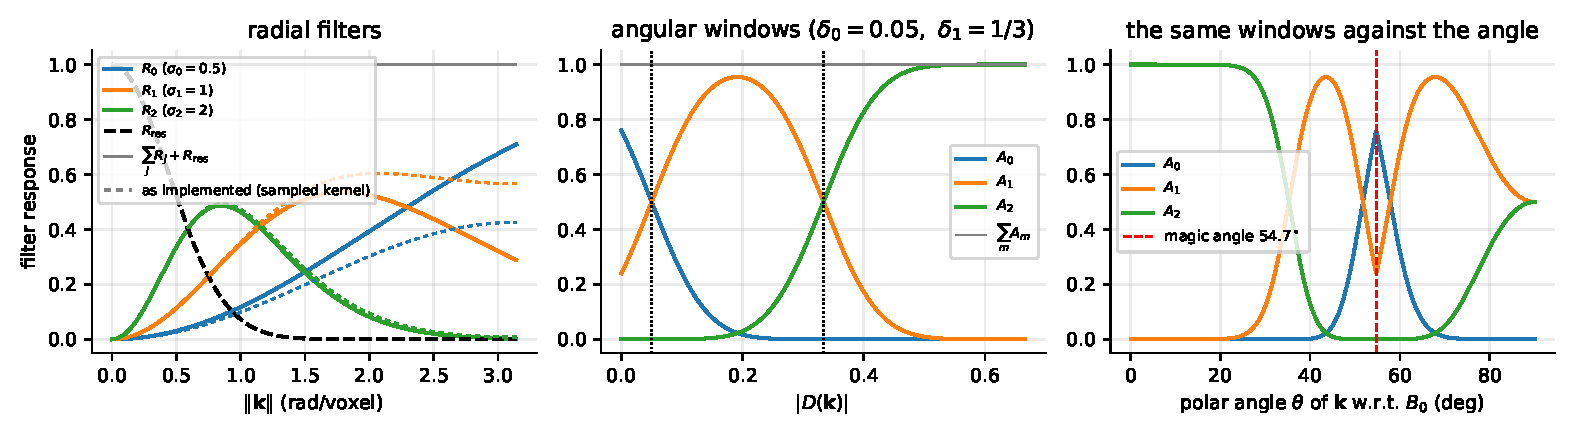
\includegraphics[width=\linewidth]{figures/fig_filters.pdf}
\caption{The Dipole-let filters actually used ($\sigma=0.5$, $J=3$; $\delta_0=0.05,\ \delta_1=1/3$, $w\approx0.100$), computed with the project code. Left: radial filters and the low-pass residual (solid: analytic $R_j$ of \eqref{eq:radial}; dashed: as implemented, with the sampled and truncated Gaussian, one axis). The curves nearly coincide for the coarse scale and differ near Nyquist for the two finest ones.
Middle: angular windows against $\abs{D}$. Right: the same windows against the polar angle of $\bk$ (the dashed line is the magic angle).}
\label{fig:filters}
\end{figure}
\begin{figure}[t]
\centering
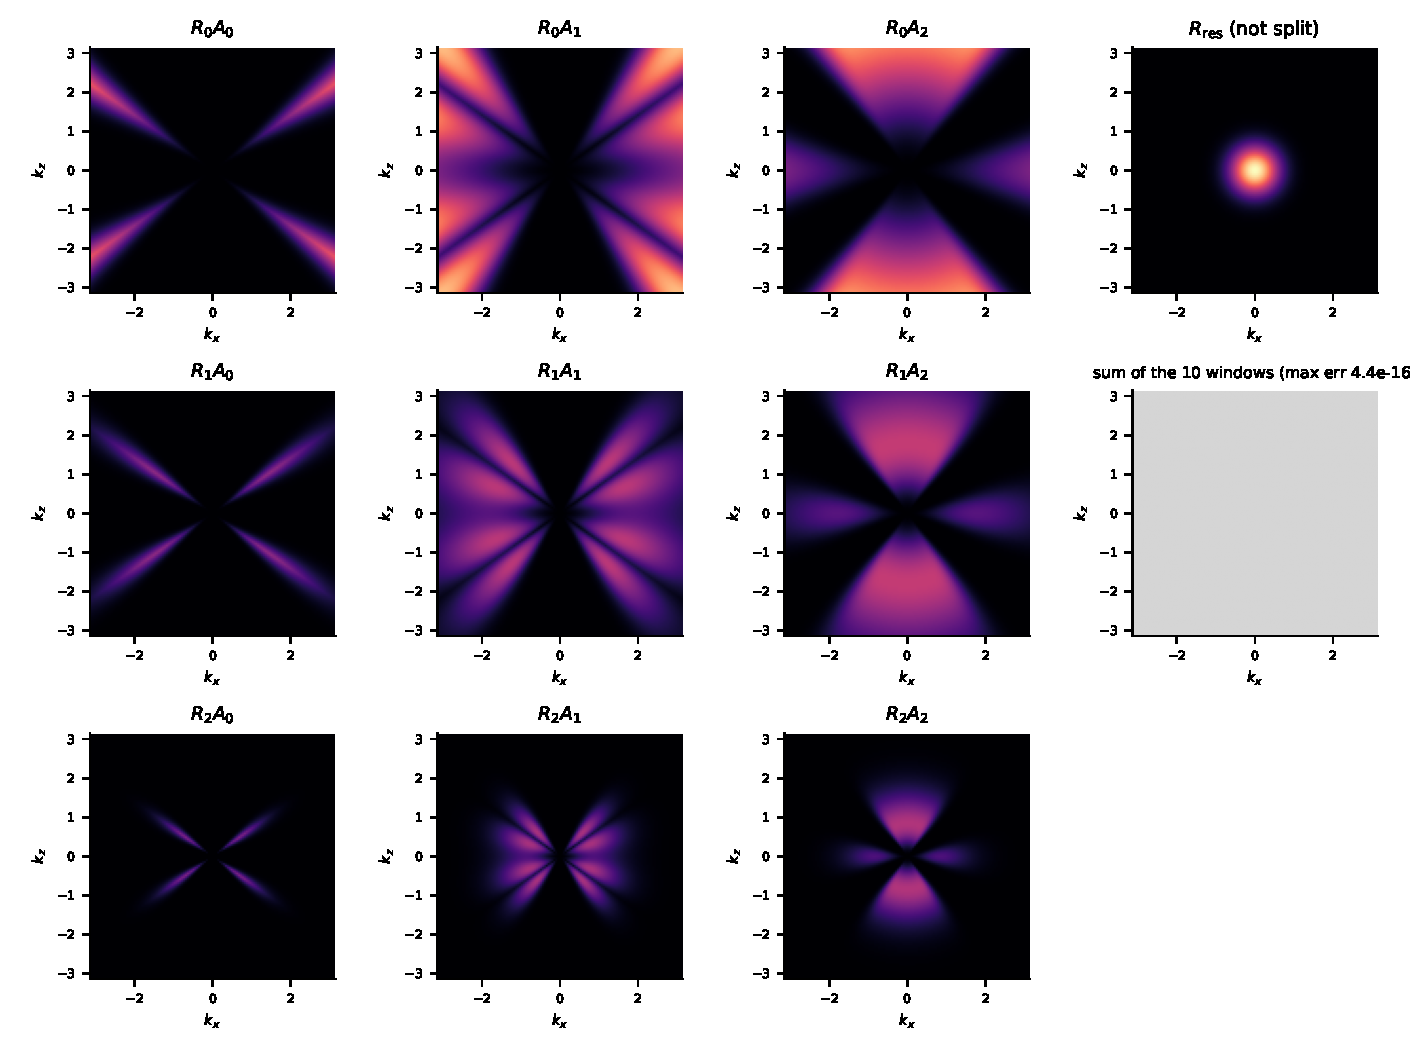
\includegraphics[width=0.78\linewidth]{figures/fig_kspace_segments.pdf}
\caption{The ten windows $\Omega_s=R_jA_m$ in the $(k_x,k_z)$ plane ($k_y=0$), and the residual $R_{\mathrm{res}}$ (top right). Their sum is identically one (centre right panel shows the sum; maximum deviation $4\cdot10^{-16}$).}
\label{fig:kspace}
\end{figure}

% =====================================================================
\section{The network}\label{sec:arch}

\subsection{Overview}
Let $C=16$ be the channel width, $L=4$ the number of spectral blocks. For a volume with measured field $\psi$ (ppm), mask $m$, weight $w$, and voxel size $h$ (a per-volume argument), with a constant input scale $s>0$:
\begin{align}
u&=\big[\psi/s,\ m,\ w\big]\in\R^{3\times\Omega}, \label{eq:input}\\
v^{(0)}&=\GELU\Big(\sum_{\kappa\in\{1,3,5,7\}}K_\kappa\star u\Big)\in\R^{C\times\Omega}, \label{eq:lift}\\
v^{(0)}&\leftarrow v^{(0)}+\GELU\big(K'_d\star_d v^{(0)}\big),\quad d=1,2,4 \ \ (\text{three residual dilated convolutions}), \label{eq:spatial}\\
v^{(\ell)}&=B_\ell\big(v^{(\ell-1)}\big),\quad\ell=1,\dots,L, \label{eq:blocks}\\
\widehat\psi_N&=s\,H v^{(L)},\qquad \widehat\psi_D=m\odot\big(\psi-\widehat\psi_N\big). \label{eq:head}
\end{align}
$K_\kappa$ are $\kappa^3$ convolutions ($3\to C$ channels, zero padding), $K'_d$ are $3^3$ convolutions with dilation $d$ ($C\to C$), $H$ is a $1\times1\times1$ convolution ($C\to1$), \emph{zero-initialised}. The scale $s$ is a stored constant (the standard deviation of the clean in-mask field, $0.0084$\,ppm for RC1).
\Cref{fig:arch} sketches the data flow.

\begin{figure}[t]
\centering
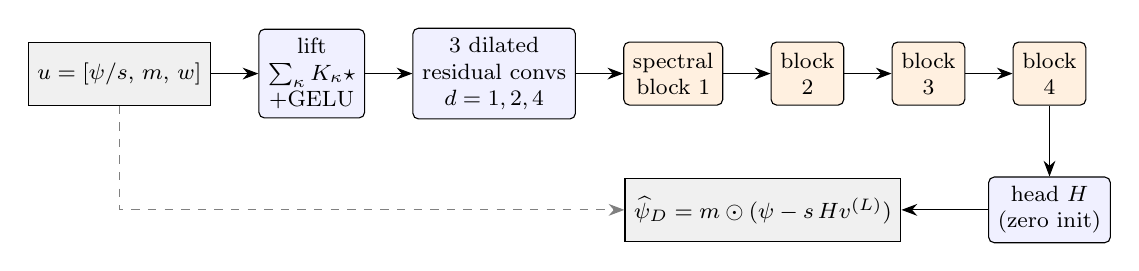
\begin{tikzpicture}[node distance=5mm and 6mm,
 box/.style={draw,rounded corners=2pt,minimum height=8mm,align=center,font=\footnotesize,fill=blue!6},
 sp/.style={draw,rounded corners=2pt,minimum height=8mm,align=center,font=\footnotesize,fill=orange!12},
 io/.style={draw,minimum height=8mm,align=center,font=\footnotesize,fill=gray!12},
 arr/.style={-{Stealth[length=2mm]}}]
 \node[io] (in) {$u=[\psi/s,\,m,\,w]$};
 \node[box,right=of in] (lift) {lift\\$\sum_\kappa K_\kappa\star$\\+GELU};
 \node[box,right=of lift] (sp) {3 dilated\\residual convs\\$d=1,2,4$};
 \node[sp,right=of sp] (b1) {spectral\\block 1};
 \node[sp,right=of b1] (b2) {block\\2};
 \node[sp,right=of b2] (b3) {block\\3};
 \node[sp,right=of b3] (b4) {block\\4};
 \node[box,below=9mm of b4] (hd) {head $H$\\(zero init)};
 \node[io,left=of hd,xshift=-5mm] (out) {$\widehat\psi_D=m\odot(\psi-s\,Hv^{(L)})$};
 \draw[arr] (in)--(lift); \draw[arr] (lift)--(sp); \draw[arr] (sp)--(b1); \draw[arr] (b1)--(b2); \draw[arr] (b2)--(b3); \draw[arr] (b3)--(b4);
 \draw[arr] (b4)--(hd); \draw[arr] (hd)--(out);
 \draw[arr,dashed,gray] (in.south) |- (out.west);
\end{tikzpicture}
\caption{Data flow of the cleaner. The dashed line is the skip: $\psi$ enters the output directly. All tensors have $C=16$ channels between the lift and the head. Local receptive radius: $3+1+2+4=10$ voxels; every spectral block is global.}
\label{fig:arch}
\end{figure}

\subsection{The Dipole-let spectral block}
\paragraph{Segment operator.} For a multichannel field $v\in\R^{C\times\Omega}$ and $s\in\mathcal S$ let
\begin{equation}
\mathcal S_sv\;:=\;\F\,\md_s v\;=\;\Omega_s\cdot\F v\ \in\C^{C\times\Omega}\qquad(\text{channel-wise}),
\end{equation}
the Fourier transform of the $s$-th Dipole-let coefficient. In the code this is computed as in \cref{sec:dipolelets} (image-domain radial cascade, FFT, multiplication by $A_m$).

\paragraph{Block.} Block $\ell$ has, for each segment $s$, a complex mixing matrix $P_{\ell,s}\in\C^{C\times C}$, a $1\times1\times1$ skip convolution $(W_\ell,b_\ell)$, and a small gain network producing scalar fields $g_{\ell,s}(\bk)$:
\begin{equation}\label{eq:block}
\boxed{\,B_\ell(v)=v+\GELU\Big(W_\ell v+b_\ell+\Real\,\F^{-1}\Big[\sum_{s\in\mathcal S}g_{\ell,s}(\bxi)\,P_{\ell,s}\,\mathcal S_sv\Big]\Big)\,}
\end{equation}
\begin{equation}\label{eq:gain}
g_{\ell,s}(\bxi)=1+\Big[V^{(2)}_\ell\,\GELU\big(V^{(1)}_\ell\,\phi(\bxi)+c^{(1)}_\ell\big)+c^{(2)}_\ell\Big]_s,\qquad
\phi(\bxi)=\Big(D(\bxi),\ 2\norm{\bxi}_2,\ \bxi/\norm{\bxi}_2\Big)\in\R^5,
\end{equation}
where $V^{(1)}\in\R^{16\times5}$, $V^{(2)}\in\R^{S\times16}$ act pointwise in $\bxi$ (two $1\times1\times1$ convolutions on the feature volume $\phi$; $\norm\bxi$ in cycles/mm, so the gain is voxel-size aware), and $V^{(2)},c^{(2)}$ are zero-initialised so that $g\equiv1$ at the start.
Without $k$-conditioning $g_{\ell,s}\equiv1$.

\paragraph{Fourier-multiplier view.} Writing $V=\F v$, the spectral term of \eqref{eq:block} is $\Real\,\F^{-1}[T_\ell(\bxi)V(\bxi)]$ with the matrix-valued \emph{symbol}
\begin{equation}\label{eq:symbol}
T_\ell(\bxi)=\sum_{s\in\mathcal S}g_{\ell,s}(\bxi)\,\Omega_s(\bxi)\,P_{\ell,s}\ \in\C^{C\times C}.
\end{equation}
A Fourier neural operator layer \cite{fno} is $v\mapsto\sigma\big(Wv+\F^{-1}[R(\bk)\F v]\big)$ with a free matrix $R(\bk)$ per retained mode (modes are truncated). Here $R$ is not free: it is a combination of
only $S=10$ matrices, interpolated over $\bk$ by the Dipole-let partition of unity and modulated by scalar functions of $(D,\norm\bxi,\hat\bxi)$. No mode is truncated. Thus the block has $S\cdot2C^2+O(C)=5{,}658$
parameters instead of $2C^2N$, and its symbol is constant (up to the smooth gain) on each cell of the partition of $k$-space that separates scales and distance to the magic cone.

\begin{figure}[t]
\centering
\resizebox{\linewidth}{!}{%
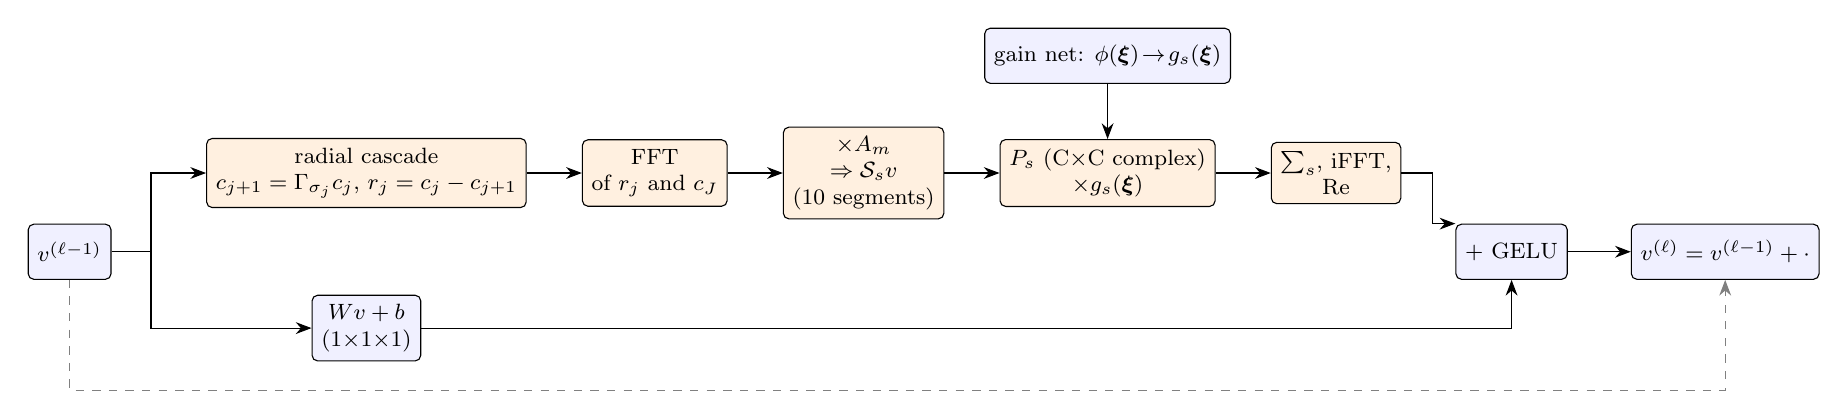
\begin{tikzpicture}[node distance=5mm and 7mm,
 box/.style={draw,rounded corners=2pt,minimum height=7mm,align=center,font=\footnotesize,fill=blue!6},
 sp/.style={draw,rounded corners=2pt,minimum height=7mm,align=center,font=\footnotesize,fill=orange!12},
 arr/.style={-{Stealth[length=2mm]}}]
 \node[box] (v) {$v^{(\ell-1)}$};
 \node[sp,right=12mm of v,yshift=10mm] (casc) {radial cascade\\$c_{j+1}=\Gamma_{\sigma_j}c_j$,\ $r_j=c_j-c_{j+1}$};
 \node[sp,right=of casc] (fft) {FFT\\of $r_j$ and $c_J$};
 \node[sp,right=of fft] (win) {$\times A_m$\\$\Rightarrow\mathcal S_{s}v$\\(10 segments)};
 \node[sp,right=of win] (mix) {$P_s$ (C$\times$C complex)\\$\times g_s(\bxi)$};
 \node[sp,right=of mix] (sum) {$\sum_s$, iFFT,\\$\Real$};
 \node[box,below=11mm of casc] (skip) {$W v+b$\\(1$\times$1$\times$1)};
 \node[box] (add) at ($(sum.east)+(14mm,-10mm)$) {$+$\ GELU};
 \node[box,right=8mm of add] (out) {$v^{(\ell)}=v^{(\ell-1)}+\cdot$};
 \node[box,above=7mm of mix] (gain) {gain net: $\phi(\bxi)\!\to\!g_s(\bxi)$};
 \draw[arr] (v.east)--++(5mm,0)|-(casc.west);
 \draw[arr] (v.east)--++(5mm,0)|-(skip.west);
 \draw[arr] (casc)--(fft); \draw[arr] (fft)--(win); \draw[arr] (win)--(mix); \draw[arr] (mix)--(sum);
 \draw[arr] (gain)--(mix);
 \draw[arr] (sum.east)--++(4mm,0)|-(add.north west);
 \draw[arr] (skip.east)-|(add.south);
 \draw[arr] (add)--(out);
 \draw[arr,dashed,gray] (v.south)--++(0,-14mm)-|(out.south);
\end{tikzpicture}}
\caption{One spectral block, \eqref{eq:block}. The Dipole-let segments give the cells of the frequency domain; each cell has its own complex channel mixing, modulated by a gain depending on the physical frequency.}
\label{fig:block}
\end{figure}

\subsection{Properties}
\begin{proposition}[Partition of unity and exact analysis]\label{prop:pou}
$\sum_{s}\Omega_s\equiv1$. Hence, if $P_{\ell,s}=P$ for all $s$ and $g\equiv1$, the spectral term equals $(\Real P)\,v$ (a $1\times1\times1$ convolution) and $B_\ell(v)=v+\GELU((W_\ell+\Real P)v+b_\ell)$.
\end{proposition}
\begin{proof}
$\sum_s\Omega_s=\sum_{j,m}R_jA_m+R_{\mathrm{res}}=(\sum_jR_j)(\sum_mA_m)+R_{\mathrm{res}}=\sum_jR_j+R_{\mathrm{res}}=1$. With constant symbol $T=P$, $\Real\,\F^{-1}[P\,V]=\Real(P\,v)=(\Real P)v$ for real $v$. \qedhere
\end{proof}
(Numerical check: the difference between the block and $v+\GELU(Pv)$ is $9.5\cdot10^{-7}$ in float32.) The block therefore \emph{contains} an ordinary residual convolutional block as a special case.

\begin{proposition}[Identity at initialisation]\label{prop:id}
At initialisation $H=0$, hence $\widehat\psi_N=0$ and $f_\theta(\psi,m,w)=m\odot\psi$ for every input, independently of all other weights. The gain networks also start at $g\equiv1$.
\end{proposition}
This is verified exactly (error $0.0$) for the Dipole-let model and for the single-segment ablation. It guarantees that training starts from the baseline ``dirty field inside the mask'' and that any gain is relative to it.

\begin{proposition}[Real-valuedness and inert parameters]\label{prop:real}
For real $v$, $V=\F v$ satisfies $V(-\bxi)=\overline{V(\bxi)}$ and
\[
\Real\,\F^{-1}[TV]=\F^{-1}\!\big[T_h V\big],\qquad T_h(\bxi)=\tfrac12\big(T(\bxi)+\overline{T(-\bxi)}\big).
\]
The windows $\Omega_s$ are even in $\bxi$ ($R_j$ depends on $\norm\bk$, $A_m$ on $\abs D$). Consequently
\[
T_h(\bxi)=\sum_s\Omega_s(\bxi)\Big[\Real P_s\;\tfrac{g_s(\bxi)+g_s(-\bxi)}2+\,i\,\Imag P_s\;\tfrac{g_s(\bxi)-g_s(-\bxi)}2\Big].
\]
If $g\equiv1$ (no $k$-conditioning), the imaginary parts of all $P_s$ have \emph{no effect} on the output. They can matter only through the odd part of $g_s$, which is available only through the feature $\hat\bxi=\bxi/\norm\bxi$ (odd under $\bxi\to-\bxi$); $D$ and $\norm\bxi$ are even.
\end{proposition}
\begin{proof}
$\Real u=\tfrac12(u+\bar u)$ and $\overline{(TV)(\bxi)}$ transforms to $\overline{T(-\bxi)}\,\overline{V(-\bxi)}=\overline{T(-\bxi)}V(\bxi)$. Expand $T=\sum_sg_s\Omega_sP_s$ with $\Omega_s$ even. \qedhere
\end{proof}
This is not only formal: with $k$-conditioning disabled, the measured maximum gradient of the imaginary parameters was $2.8\cdot10^{-7}$ against $14.6$ for the real ones; with $k$-conditioning on it was $3.1$ against $687$.
Practical consequences: (i) in the ablation ``without $k$-conditioning'' half of the 5,120 mixing parameters per block are inert, so parameter counts are misleading there; (ii) the single-segment ablation has symbol $g(\bxi)P$ whose imaginary part acts only through the odd part of $g$.

\begin{proposition}[Shift equivariance, and its limits]\label{prop:shift}
Every operator in \eqref{eq:input}--\eqref{eq:head} is a convolution, a pointwise nonlinearity, or a Fourier multiplier whose symbol depends on $\bxi$ only. Hence $f_\theta$ commutes with periodic translations of $(\psi,m,w)$, except for (a) the zero padding of the convolutions and the mirror boundary of $\Gamma_\sigma$, which act within a distance $10$ voxels (convolutions) and $\lceil4\sigma_j\rceil\le8$ voxels (smoothing) of the border, and (b) the dependence of the windows on the volume shape through the frequency grid.
\end{proposition}
Consequences: the model is fully convolutional, trained on $96^3$ patches and applied to whole volumes of other shapes ($160^3$, $164\times205\times205$) with the same weights; windows and features are rebuilt per (shape, voxel size).

\begin{remark}[Receptive field]
The local branch (lift $7^3$, dilated $3^3$ with $d=1,2,4$) has radius $3+1+2+4=10$ voxels. At random initialisation, $95\%$ of the gradient mass of one output voxel with respect to the input lies within $7$ voxels and $98.5\%$ within $10$ (measured at $48^3$);
long-range interaction is available only through the Fourier branch and will matter only if training makes the $P_{\ell,s}$ and gains large. Two thirds of the parameters (44{,}656 of 67{,}305) sit in the local convolutions.
\end{remark}

\subsection{Parameter inventory}
\begin{table}[h]
\centering
\begin{tabular}{@{}llrl@{}}
\toprule
Module & Parameters & Count & Derivation \\
\midrule
Lift $K_1,K_3,K_5,K_7$ & weights + bias & 23{,}872 & $\sum_\kappa(3C\kappa^3+C)=64+1312+6016+16480$ \\
Dilated convs $d=1,2,4$ & weights + bias & 20{,}784 & $3\times(27C^2+C)$ \\
Block mixing $P_s$ (re+im) & $S\cdot2C^2$ & $4\times5{,}120$ & $10\cdot2\cdot256$ per block \\
Block gain net & $5\!\to\!16\!\to\!S$ & $4\times266$ & $5\cdot16+16+16\cdot10+10$ \\
Block skip $1\times1\times1$ & $C^2+C$ & $4\times272$ & \\
Head $H$ & $C+1$ & 17 & \\
\midrule
\textbf{Total} & & \textbf{67{,}305} & single-segment ablation: 48{,}261 \\
\bottomrule
\end{tabular}
\caption{Parameter inventory (measured and derived agree).}
\end{table}

\paragraph{Plain-FNO ablation.} The code has a switch \code{plain=True} that replaces the Dipole-let partition by a single segment (the whole spectrum, $S=1$): symbol $g(\bxi)P$. This isolates the effect of the partition but is not a parameter-matched
Fourier network (48{,}261 vs 67{,}305 parameters; a matched version would use more channels).

% =====================================================================
\section{Training data}\label{sec:data}

\subsection{Sources}
\begin{table}[h]
\centering\small
\begin{tabularx}{\linewidth}{@{}p{2.0cm}p{3.3cm}p{1.7cm}Xp{1.9cm}@{}}
\toprule
 & Grid / voxel & $B_0$, TE & Content & Role \\
\midrule
RC1 (FANSI data) & $160^3$, $1.0625\times1.0625\times1.0714$\,mm & 2.89\,T, 25\,ms & COSMOS $\chi$, STI tensors, magnitude, mask, real tissue phase & training (one head) \\
Sim2 (RC2) & $164\times205\times205$, 0.999\,mm & 7\,T, 8\,ms & ground-truth $\chi$, dirty frequency map, 4 echoes, mask & test target only \\
AHEAD \cite{ahead} & $234\times320\times320$, $0.70\times0.64\times0.64$\,mm & 7\,T & processed QSM, R2*, T1w, 105 subjects (copied to the server) & planned (S4c) \\
\bottomrule
\end{tabularx}
\caption{Data sets. AHEAD is stored but not used yet; it contains processed QSM maps rather than raw phase, so all its artifacts would be synthetic and its ``clean'' target would be a reconstruction rather than COSMOS.}
\end{table}
Sim2 is \emph{never} used for training or for selecting a checkpoint; it is evaluated every 250 steps as a monitoring curve and at the end.

\subsection{Clean target and pairs}
For RC1, $\chi$ is the COSMOS map minus its mean and $y=m\odot\psi_D(\chi)$ by \eqref{eq:forward} with the RC1 voxel size. A training example is $(x,m,w,y)$ with $x$ the corrupted field of one artifact family, $w$ the (real) magnitude, and all four tensors cropped from the same $96^3$ window.

\subsection{Artifact families}
With $\phi=\phi_{\mathrm{TE}}$ and the real RC1 magnitude $M\in[0,1]$:
\begin{description}[leftmargin=1.2em,itemsep=2pt]
\item[noise] (notebook exp2/3) $\ \tilde s=M e^{i\phi\psi_D}+\mathrm{SNR}^{-1}(\epsilon_1+i\epsilon_2)$, $\epsilon_{1,2}\sim\mathcal N(0,1)$, $\ \tilde\psi=\arg(\tilde s)/\phi$ inside the mask (noise-free outside). For $M\,\mathrm{SNR}\gg1$ the phase noise has standard deviation $\approx1/(\mathrm{SNR}\,M\,\phi)$ ppm; $\mathrm{SNR}$ is log-uniform in $[40,100]$ and relative to unit magnitude (local SNR is $M\cdot\mathrm{SNR}$).
\item[jumps] (exp4) $\ \tilde\psi=\psi_D+\sum_{p=1}^{n}a_p\,\delta_{\bx_p}$, $n\sim\mathcal U\{1,\dots,6\}$, $a_p\in\{\pm1,\pm2\}$ ppm, $\bx_p$ uniform in the mask. ($\psi^\star$ in the notebook.)
\item[spheres\_phase] (exp6) $\ \tilde\psi=\psi_D+\sum_pb_p\ind_{B(\bx_p,r_p)}$, $n\in\{1..4\}$, $r_p\in[3,5]$ voxels, $\abs{b_p}\in[0.2,0.45]$ ppm (notebook: $r=4$, $0.33$).
\item[cylinders] (exp5) like spheres, with cylinders of radius $\in[6,10]$ and height $\in[6,10]$ voxels, random Euler rotation, $\abs b\in[0.3,0.7]$ ppm (notebook: 8, 8, 0.5). The cylinder axis is the array axis $z$ before rotation (the notebook's \code{create\_geometric\_phantom} permutes axes; here centres and shapes are in array order).
\item[tissue] (exp7) $\ \tilde\psi=\psi_{\text{tissue}}$, the real in-vivo tissue phase of RC1 (with $y$ still the COSMOS field; residual rms $0.0062$\,ppm).
\item[sti] (exp8) $\ \tilde\psi=\psi_{33}-(\psi_{13}+\psi_{23})$ with $\psi_{33}=\Real\F^{-1}[D\,\F\chi_{33}]$, $\psi_{13}=\Real\F^{-1}[\tfrac{\xi_x\xi_z}{\norm{\bxi}^2}\F\chi_{13}]$, $\psi_{23}$ analogous with $\xi_y\xi_z$.
\item[offdiag] (exp9) $\ \tilde\psi=\psi_D-(\psi_{13}+\psi_{23})$. (The notebook's $-p_Q$ alone has no signal, so it is applied to the clean field; a decision of ours.)
\item[spheres\_chi] (exp11) $\ \tilde\psi=\mathrm{Noise}\big(\psi_D+\Real\F^{-1}[D\,\F s]\big)$ with $s=\sum_pc_p\ind_{B(\bx_p,r_p)}$ spheres \emph{in the susceptibility} (so they have dipolar fields) plus the noise model.
\item[combo] (exp12, requested) $\ \tilde\psi=\mathrm{Noise}\big(\psi_D+\Real\F^{-1}[D\,\F s]\big)+\sum_pa_p\delta_{\bx_p}$: spheres in $\chi$, plus phase jumps, plus noise.
\end{description}
In every family the target remains $y=m\odot\psi_D$; spheres, cylinders and jumps are artifacts to be removed.

\paragraph{Mixture.} Family $f$ is drawn with probability $\propto$ weight: combo 3, spheres\_chi 2, noise 2, jumps 1, tissue 1, sti 1, offdiag 1, spheres\_phase 0.5, cylinders 0.5 (total 12). The weights favour the families that were closest to Sim2's $\psi$ in the gate analysis (\cref{sec:gate}).

\subsection{Anatomy augmentation}\label{sec:object}
The pair $(\chi,m,M)$ is rotated and rescaled \emph{before} the forward model, with $B_0$ fixed. With the resampling $\mathcal W_{Q,\rho}u(\bx)=u(Q\bx/\rho)$ about the grid centre (trilinear, zero outside), $Q=Q_{\mathrm{tilt}}Q_{\mathrm{cube}}$, $Q_{\mathrm{cube}}$ one of the 24 proper rotations of the cube (so $z$ may map onto $x$ or $y$),
$Q_{\mathrm{tilt}}$ an Euler rotation with each angle $\sim\mathcal U(-20^\circ,20^\circ)$ and $\rho\sim\mathcal U(0.9,1.1)$:
\[
\chi'=m'\odot\mathcal W\chi,\quad m'=\ind[\mathcal Wm>\tfrac12],\quad M'=m'\odot\mathcal WM,\quad y'=m'\odot\psi_D(\chi').
\]
This is physically valid (a head in another pose in the same scanner), unlike rotating the field. Draws that push more than $1\%$ of the brain out of the grid are redrawn. It is applied with probability $0.7$, only to the object-agnostic families (the real-$\psi$ families
\emph{tissue, sti, offdiag} are tied to the original pose and are used on original-pose samples only; runs made only of those families never rotate the head). Voxels are treated as isotropic here (RC1's $1.0625$ vs $1.0714$\,mm differ by $<1\%$).
The cube-rotation resampling is exact: each of the 24 warps equals a distinct proper \code{rot90} composition of the array (test). On the real head all 200 test draws were accepted and the brain volume changed by factors $0.73$--$1.33$ (\cref{fig:objaug}).

\paragraph{Patch-level augmentation.} Independent random flips along each axis and a random quarter-turn in the $x$--$y$ plane (these leave $D$ invariant); $z$ is never rotated onto $x$ or $y$ at the patch level.

\subsection{Hold-out and what it does and does not protect}
For checkpoint selection a slab of the head is held out: axis $0$ ($x$), train indices $[0,100)$, gap $12$, check slab $[112,160)$, containing 15\% of the brain voxels (142k). Patches come from the training range; with a hold-out the rotated heads are built from the head truncated to the training slab so that no held-out anatomy reaches them.
Two honest limits: original-pose samples still contain the \emph{dipole field} of the whole head (the field is non-local), as in the earlier S2b experiment; and there is only one brain, so the check slab estimates generalisation within one anatomy, not across subjects. Rotated heads built from the truncated head show a flat cut (\cref{fig:objaug}).

\begin{figure}[t]
\centering
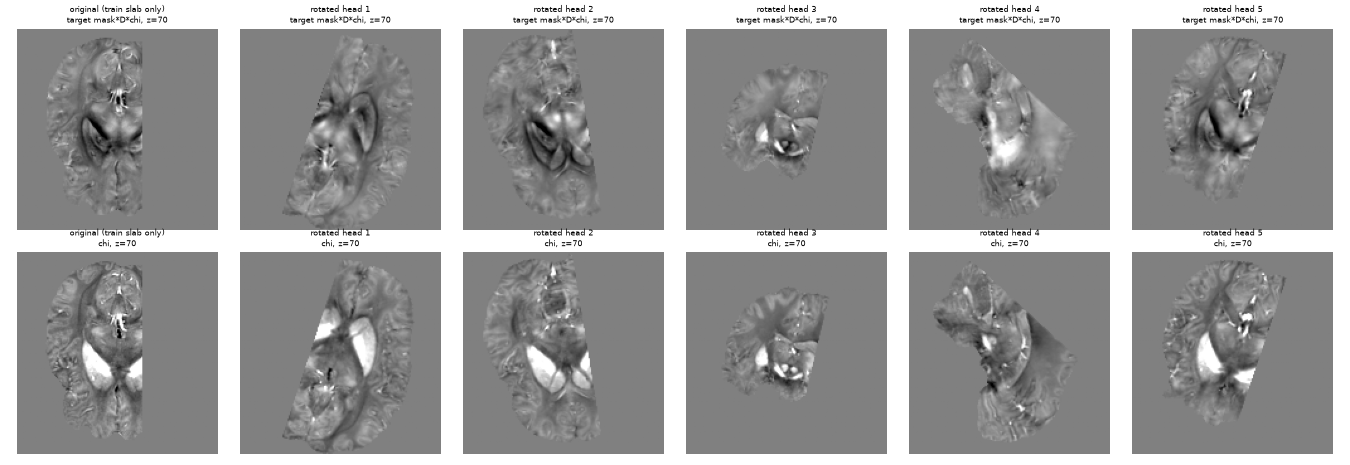
\includegraphics[width=\linewidth]{figures/object_augmentation.png}
\caption{Anatomy augmentation on RC1 (axial slice $z=70$; first column: the head truncated to the training slab, then five random draws). Top: the clean target $m\odot\psi_D(\chi')$; bottom: $\chi'$.}
\label{fig:objaug}
\end{figure}

% =====================================================================
\section{Objective, optimisation and evaluation}\label{sec:train}

\subsection{Loss}
With prediction $\widehat y=f_\theta(x,m,w)$ and target $y$, all norms taken over the whole batch,
\begin{equation}\label{eq:loss}
\mathcal L=\underbrace{\frac{\norm{m\odot(\widehat y-y)}_1}{\norm{m\odot y}_1}}_{\ell_1}+\underbrace{\frac{\norm{m\odot(\widehat y-y)}_2}{\norm{m\odot y}_2}}_{\ell_2}+\lambda_{\mathrm{cone}}\Big[E_{\Sigma}(\widehat y)-E_{\Sigma}(y)\Big]_+,\qquad
E_\Sigma(u)=\frac{\sum_{\abs{D}<\delta}\abs{\F u}^2}{\sum\abs{\F u}^2}.
\end{equation}
Currently $\lambda_{\mathrm{cone}}=0$ (the cone energy is only logged): on Sim2 only $4.8\%$ of $\psi$'s energy lies in $\abs D<0.03$ and the cone-energy cue is weak. eNDI itself is not in the loss (many iterations, data-dependent stopping).

\subsection{Optimisation}
Adam (default $\beta$'s, no weight decay), batch of 2 patches of $96^3$, base rate $\eta_0=10^{-3}$, gradient-norm clipping at 1, schedule
$\eta(t)=\eta_0\frac{t+1}{100}$ for $t<100$ and $\eta(t)=\frac{\eta_0}2\big(1+\cos\frac{\pi(t-100)}{T-100}\big)$ afterwards, $T=6000$ steps, seed 42. All runs of the S4b series share seed, steps, optimiser and hold-out.

\subsection{Selection and monitoring}
Every 250 steps the model is evaluated on full volumes with fixed draws (fixed seed) of all nine families on the original RC1 head. Let $m_T=m\odot\ind_{\text{check slab}}$ and $\mathrm{NRMSE}_T(a,y)=\norm{m_T\odot(a-y)}_2/\norm{m_T\odot y}_2$. The selection score is
\begin{equation}
\rho=\frac1{\abs{\mathcal F_{\mathrm{tr}}}}\sum_{f\in\mathcal F_{\mathrm{tr}}}\frac{\mathrm{NRMSE}_T(\widehat y_f,y)}{\mathrm{NRMSE}_T(m\odot\psi_f,y)},
\end{equation}
over the families $\mathcal F_{\mathrm{tr}}$ with positive weight (families with nothing to remove in the slab are skipped; localised artifacts of the fixed draws are placed inside the slab). $\rho<1$ means the cleaner beats the dirty field on average on held-out anatomy.
A second column averages all nine families. The \textbf{Sim2 monitoring curve} (phase NRMSE of $f_\theta$ on the full Sim2 volume against $m\odot\psi_D(\chi_{\mathrm{Sim2}})$, and the same for the dirty field) never influences training or selection; the code path of the trainer is tested to give identical weights with and without Sim2.

\subsection{Scoring with eNDI}
The final criterion is the quality of the susceptibility map obtained by the authors' \code{ndiCG\_auto} (linear, $\alpha=10^{-5}$, at most 150 iterations, automatic stopping, zero-padded to $256^3$) from three inputs with \emph{identical} settings:
the dirty field, the cleaned field, and the oracle $m\odot\psi_D$; metrics are NRMSE (\%) and XSIM against the ground truth, plus a low-pass baseline. The eNDI code is vendored unchanged.
The oracle is not a true ceiling (the true field outside the mask retains useful information). eNDI is currently run only on Sim2 (\code{score\_run.py}); an eNDI score on the RC1 check slab is not implemented.

% =====================================================================
\section{Computational method}\label{sec:compute}

\subsection{Software structure}
\begin{table}[h]
\centering\small
\begin{tabular}{@{}lp{10.5cm}@{}}
\toprule
Module & Role \\
\midrule
\code{physics.py} & dipole kernel for any shape, voxel size and $B_0$ direction; Hermitian projection \\
\code{dipolelets.py} & Dipole-let transform (starlet/Gaussian cascade, erf windows), lazy segment generator, single-segment ablation \\
\code{cleaner.py} & \code{PhaseCleaner}, \code{DipoleletBlock}, $k$-features; per-volume voxel size; nested checkpointing \\
\code{rc1.py}, \code{rc2.py} & loaders, unit conversions, STI fields \\
\code{artifacts.py} & the nine families, anatomy augmentation (\code{augment\_object}), mixture weights \\
\code{rc1\_data.py} & \code{RC1Source}: hold-out, window selection, patches, fixed draws \\
\code{rc1\_train.py} & training loop, evaluation, Sim2 monitor, resumable runs \\
\code{scoring.py} & forward model and the wrapper around the vendored eNDI \\
\bottomrule
\end{tabular}
\caption{Modules of \code{src/mcno\_qsm}.}
\end{table}

\begin{figure}[t]
\centering
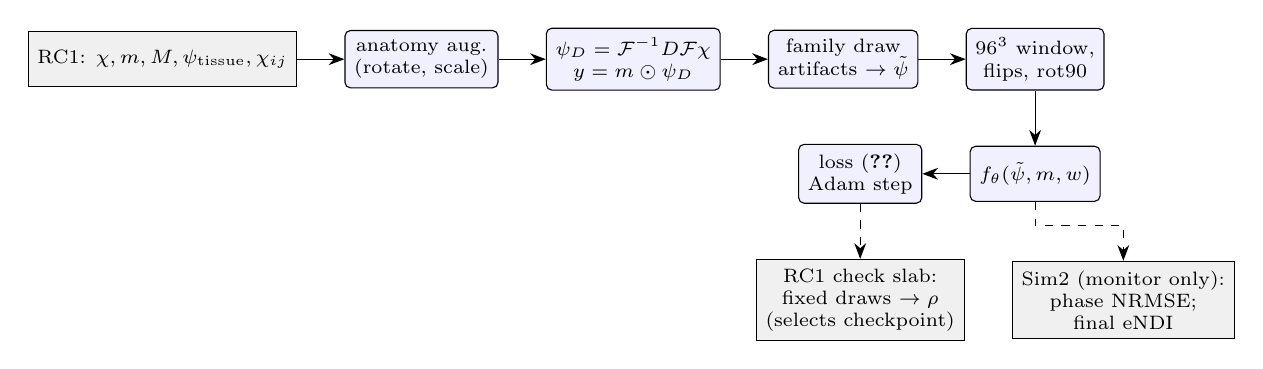
\begin{tikzpicture}[node distance=4mm and 6mm,
 box/.style={draw,rounded corners=2pt,minimum height=7mm,align=center,font=\scriptsize,fill=blue!6},
 io/.style={draw,minimum height=7mm,align=center,font=\scriptsize,fill=gray!12},
 arr/.style={-{Stealth[length=2mm]}}]
 \node[io] (rc1) {RC1: $\chi,m,M,\psi_{\mathrm{tissue}},\chi_{ij}$};
 \node[box,right=of rc1] (obj) {anatomy aug.\\(rotate, scale)};
 \node[box,right=of obj] (fwd) {$\psi_D=\F^{-1}D\F\chi$\\$y=m\odot\psi_D$};
 \node[box,right=of fwd] (art) {family draw\\artifacts $\to\tilde\psi$};
 \node[box,right=of art] (crop) {$96^3$ window,\\flips, rot90};
 \node[box,below=7mm of crop] (net) {$f_\theta(\tilde\psi,m,w)$};
 \node[box,left=of net] (loss) {loss \eqref{eq:loss}\\Adam step};
 \node[io,below=7mm of loss] (chk) {RC1 check slab:\\fixed draws $\to\rho$\\(selects checkpoint)};
 \node[io,right=of chk] (sim) {Sim2 (monitor only):\\phase NRMSE;\\final eNDI};
 \draw[arr] (rc1)--(obj); \draw[arr] (obj)--(fwd); \draw[arr] (fwd)--(art); \draw[arr] (art)--(crop); \draw[arr] (crop)--(net); \draw[arr] (net)--(loss);
 \draw[arr,dashed] (loss)--(chk); \draw[arr,dashed] (net.south)--++(0,-3mm)-|(sim.north);
\end{tikzpicture}
\caption{Training data flow (S4b). Sim2 only enters the evaluation branch.}
\end{figure}

\subsection{Algorithms}
\begin{algorithm}[h]
\caption{Forward pass of one spectral block on a $C\times N_x\times N_y\times N_z$ tensor}
\begin{algorithmic}[1]
\Require $v$, windows $\{A_m\}$ and features $\phi$ for this (shape, voxel size), parameters $\{P_s\},W,b$, gain net
\State $g\gets 1+\text{gain-net}(\phi)$ \Comment{$S$ scalar fields}
\State $c_0\gets v$;\ $\mathrm{total}\gets0$;\ $s\gets0$
\For{$j=0,\dots,J-1$}
  \State $c_{j+1}\gets\Gamma_{\sigma_j}c_j$;\ $\widehat r\gets\F(c_j-c_{j+1})$ \Comment{one FFT per scale, shared by the $M$ bands}
  \For{$m=0,\dots,M-1$}
    \State $\mathrm{total}\mathrel{+}=g_s\cdot P_s\,(A_m\widehat r)$;\ $s\gets s+1$ \Comment{recomputed in backward (segment checkpoint)}
  \EndFor
\EndFor
\State $\mathrm{total}\mathrel{+}=g_s\cdot P_s\,\F(c_J)$ \Comment{residual segment}
\State \Return $v+\GELU\big(Wv+b+\Real\,\F^{-1}(\mathrm{total})\big)$
\end{algorithmic}
\end{algorithm}

\begin{algorithm}[h]
\caption{One training sample (\code{RC1Source.patch})}
\begin{algorithmic}[1]
\State draw $r\sim\mathcal U(0,1)$; $\textit{rotate}\gets$ [there is an object-agnostic family and $r<0.7$]
\If{\textit{rotate}} $V\gets$ \Call{AugmentObject}{training head} \Comment{may fail $\Rightarrow$ original head}\EndIf
\State pick the family $f$ from the weights (restricted to object-agnostic ones if the head was rotated)
\State pick a window origin with mask share $>5\%$ (training slab only if the head is not rotated)
\State $\tilde\psi\gets\textsc{MakeDirty}(f,V,\text{region}=\text{window})$ \Comment{full-volume FFTs; artifacts centred inside the window}
\State crop $(\tilde\psi,m,w,y)$, apply random flips and quarter-turn \State \Return the tensors
\end{algorithmic}
\end{algorithm}

\subsection{Cost model}
Let $N$ be the number of voxels of the tensor being processed. A spectral block performs $J+1=4$ forward and $1$ inverse FFT of $C$ channels ($\mathcal O(5\,CN\log N)$), $J=3$ separable Gaussian smoothings ($\mathcal O(CN\sum_j(2\lceil4\sigma_j\rceil+1)\cdot3)$, i.e.\ $5,9,17$ taps per axis for $\sigma_j=0.5,1,2$),
and $S$ windowed complex channel mixings ($\mathcal O(SC^2N)$ complex multiply-adds, $S=10$). The local branch costs $3C\big(\sum_\kappa\kappa^3\big)N+3\cdot27\,C^2N$ multiply-adds. These are operation counts only; wall-clock time on the GPU is memory-bandwidth bound and is measured, not predicted (below).

\paragraph{Memory.} Parameters and Adam state are below 1\,MB. Activations dominate. One complex spectrum of $C$ channels is $8CN$ bytes ($113$\,MB at $96^3$ with $C=16$), a real tensor $4CN$ bytes. Without checkpointing, a block keeps on the order of $S$ such spectra alive for backward (the windowed segments and their products with the mixing matrices); this is a reasoning aid, the measured peaks below are what counts.
Two nested \code{torch.utils.checkpoint} levels \cite{checkpoint} cut this: the outer level stores only the input of each block and recomputes the block in backward; the inner level (added in this work) stores only the shared scale spectra and recomputes each segment's window, mixing and gain.
Measured peak GPU memory of one training step on the shared RTX 5090 (32\,GB; $C=16$, fp32):

\begin{table}[h]
\centering
\begin{tabular}{@{}lrrrr@{}}
\toprule
patch / batch & $96^3$/1 & $96^3$/2 & $112^3$/2 & $128^3$/2 \\
\midrule
block checkpoint only (GB) & 4.28 & 8.58 & 13.61 & 20.24 \\
+ per-segment checkpoint (GB) & \textbf{2.68} & \textbf{5.10} & \textbf{8.08} & \textbf{12.00} \\
\bottomrule
\end{tabular}
\caption{Peak GPU memory of a training step (measured with \code{scripts/measure\_memory.py}). A full S4b step at $96^3$/2 including the full-volume evaluation peaked at 8.6\,GB in the smoke test.}
\end{table}
\begin{figure}[h]
\centering
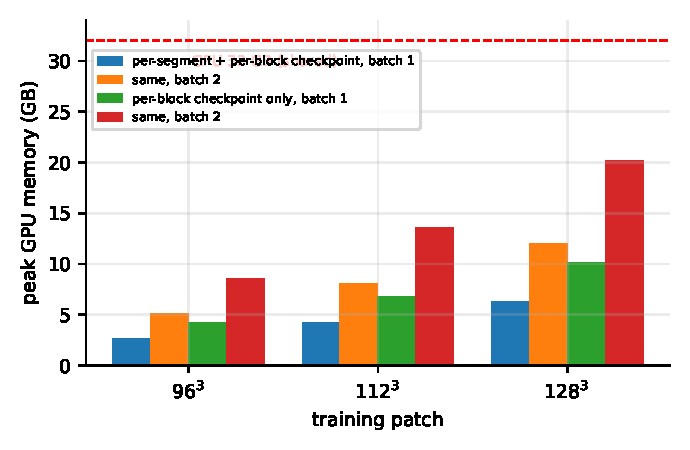
\includegraphics[width=0.55\linewidth]{figures/fig_memory.pdf}
\caption{Memory with and without the inner checkpoint level.}
\end{figure}
The extra recomputation costs additional time per step; its exact value for the final configuration is to be measured during S4b (the earlier un-nested model ran at $0.23$\,s/step at $96^3$/1; a $20$-step smoke test including one full evaluation took $14.8$\,s).
Per-sample anatomy augmentation on the GPU costs about $0.01$\,s (including artifact generation), against a step of a few tenths of a second.

\paragraph{Numerical precision.} All training is fp32. Lower precision would not help much here: the dominant tensors are complex spectra, half-precision FFTs on CUDA are restricted (to power-of-two sizes in PyTorch; our sizes $96,160,164,205$ are not), the model is tiny and memory-bound rather than compute-bound,
and 8-bit formats are designed for matrix multiplies, not for FFTs or $3^3$ convolutions with $16$ channels. The field itself is tiny in ppm ($\psi$ rms $\sim10^{-2}$, artifacts $\sim4\cdot10^{-3}$), which is another reason for the input scale $s$.
These statements are design arguments; reduced-precision training was not tested.

\subsection{Reproducibility, resumption and tests}
\begin{itemize}[leftmargin=1.5em,itemsep=1pt]
\item Three random streams: a NumPy \code{Generator} (family, window, placements, rotations), a device \code{torch.Generator} (noise), and the global torch seed (initialisation). Their states, the optimiser and the step are saved in \code{last.pt} every 250 steps; a resumed run reproduces the uninterrupted weights (test, tolerance $10^{-6}$). The same seed yields identical patches (test). GPU kernels are not guaranteed bitwise-deterministic.
\item Every run writes a new folder with configuration, data hashes, parameter count, device and library versions, \code{eval.csv}, \code{best.pt}, and \code{DONE}/\code{FAILED}.
\item 76 automated tests (all passing on the laptop and the server): Dipole-let equivalence to the reference ($10^{-9}$), kernel alignment for odd sizes, identity at initialisation, gradient flow to every parameter, checkpointed gradients equal to non-checkpointed ones,
exactness of the 24 cube rotations, geometry of balls and cylinders, STI fields against a literal transcription of the notebook, hold-out truncation, mixture frequencies, that the training source opens no RC2 file, that Sim2 does not change the trained weights, and resumption.
\item Server runs use \code{nohup} (not \code{tmux}); the project is on a shared GPU, so memory was measured and kept below $9$\,GB.
\end{itemize}

% =====================================================================
\section{What has been found so far}\label{sec:results}

\subsection{Sim2's non-dipolar part (S0)}
Measured with the aligned kernel: $\psi_{\mathrm{Sim2}}-\psi_D$ has rms $0.0037$\,ppm against $0.0088$ for the clean field ($\norm{\cdot}/\norm{\text{dirty}}=0.39$), $84.7\%$ of its energy at $\norm\bxi>0.2$ cycles/mm, $0.13\%$ below $0.02$ and $4.8\%$ in $\abs D<0.03$ (which occupies $7.3\%$ of $k$-space); the cone-energy fraction is $1.04\%$ for the dirty field against $0.35\%$ for the clean one.
So on Sim2 the artifact is mostly rough, noise-like and is not concentrated at the mask boundary; the cone cue is weak.

\subsection{Single-volume fit and the first held-out test (S2)}
\begin{table}[h]
\centering\small
\begin{tabular}{@{}lrrr@{}}
\toprule
\multicolumn{4}{l}{\textbf{S2a} --- trained and scored on the same Sim2 volume (a fit, not a result of the method)} \\
 & phase NRMSE & eNDI NRMSE & XSIM \\
\midrule
dirty & 42.24\% & 50.87\% & 0.515 \\
low-pass $\sigma=0.5$ & 28.99\% & 49.03\% & 0.525 \\
cleaned (masked) & 10.39\% & 45.79\% & 0.557 \\
oracle (clean in mask) & 0\% & 44.22\% & 0.583 \\
\midrule
\multicolumn{4}{l}{\textbf{S2b} --- trained on the first 60\% of one axis, tested on a slab never seen (gap 16)} \\
\midrule
dirty & 65.29\% & 64.10\% & -- \\
low-pass & 58.44\% & 63.17\% & -- \\
cleaned & 54.73\% & \textbf{65.45\%} (worse than dirty) & -- \\
oracle & 0\% & 59.20\% & -- \\
\bottomrule
\end{tabular}
\caption{Earlier single-volume experiments (Sim2 only; single volume, single seed). In S2b the fresh-noise test error was lowest after about 500 steps and then rose while the training error kept falling: the network memorised one brain. Training only on simulated noise (never seeing the real $\psi$) gave the same behaviour, so the real noise realisation is not the cause; the likely cause is the lack of anatomical diversity (not proven).}
\end{table}

\subsection{Training-set gate for the RC1 plan (S4a)}\label{sec:gate}
Statistics of $\psi=m\odot\tilde\psi-y$ for each family on RC1 (4 draws; one for the real families), compared with Sim2's measured $\psi$ ($\mathrm{rms}=0.00372$, $84.7\%$ above $0.2$ cycles/mm, $p_{99.9}\abs\psi=0.040$ ppm):
\begin{table}[h]
\centering\small
\begin{tabular}{@{}lrrrr@{}}
\toprule
family & rms (ppm) & energy $>0.2$ cyc/mm & $p_{99.9}\abs\psi$ (ppm) & remark \\
\midrule
Sim2 $\psi$ (reference) & 0.0037 & 84.7\% & 0.040 & \\
noise & 0.0040 & 96\% & 0.020 & too white \\
jumps & 0.0035 & 96\% & 0 & a few exact impulses \\
cylinders & 0.033 & 12.6\% & 0.61 & $9\times$ too large \\
spheres\_phase & 0.011 & 18\% & 0.17 & $3\times$ too large \\
tissue (real) & 0.0062 & 52\% & 0.039 & smoother \\
sti & 0.0038 & 32\% & 0.023 & smoother \\
offdiag & 0.0054 & 36\% & 0.029 & smoother \\
spheres\_chi & 0.0047 & 75\% & 0.039 & closer \\
\textbf{combo} & 0.0056 & 82\% & 0.039 & \textbf{closest} \\
\bottomrule
\end{tabular}
\caption{Artifact statistics against Sim2 (laptop CPU, 2026-10-20). The SNR that matches Sim2's $\psi$ rms with the RC1 magnitude is $59$, inside the sampled range $[40,100]$.}
\end{table}
\begin{figure}[t]
\centering
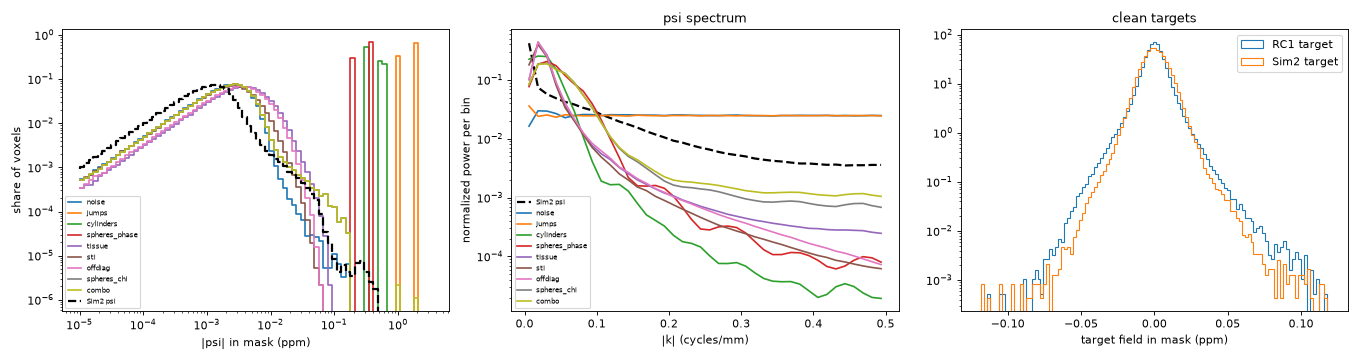
\includegraphics[width=\linewidth]{figures/histograms_spectra.png}
\caption{Left: distribution of $\abs\psi$ in the mask per family and for Sim2. Middle: radially averaged $\psi$ spectrum (each normalised by its own total). Right: histograms of the clean targets of RC1 and Sim2 (similar in range).}
\end{figure}
\paragraph{Diversity, honestly.} RC1 is one head and one real $\psi$. A $96^3$ patch of it contains $58\%$ brain on average, so patches overlap strongly; flips and in-plane rotations give 32 variants of the same anatomy. Artifacts are essentially unlimited but are not new anatomy.
The anatomy augmentation of \cref{sec:object} adds new poses and scales, not new brains; AHEAD (105 in-vivo heads) would add real anatomical variety and is deferred to S4c.

\subsection{Status of the RC1 experiments (S4b)}
Eleven runs were trained on RC1 only (seven single-family runs, exp12 alone, the mixture, and two further seeds of the mixture; $6000$ steps each, seed $42$ unless stated).
The checkpoint of each run was chosen on the RC1 check slab only; Sim2 was used for monitoring and for the final eNDI score, never for training or selection.
\Cref{tab:s4b} gives the Sim2 results (single volume; eNDI = \code{ndiCG\_auto}, $\alpha=10^{-5}$, 150 iterations at most; masked protocol).
\begin{table}[h]
\centering\small
\begin{tabular}{lrrrr}
\hline
run / baseline & phase NRMSE & eNDI NRMSE & XSIM & stop \\ \hline
dirty (masked) & 42.24\% & 52.60\% & 0.497 & 16 \\
low-pass $\sigma=0.5$ (tuned on Sim2) & 28.99\% & 49.03\% & 0.525 & 16 \\
oracle (clean in mask) & 0\% & 44.22\% & 0.583 & 20 \\ \hline
noise, seeds 42/43/44 & 26.3/26.6/26.0\% & \textbf{46.96/47.01/46.92\%} & 0.556/0.552/0.555 & 27/29/27 \
\quad mean $\pm$ sd (population) & $26.3\pm0.2$\% & $\mathbf{46.96\pm0.04}$\% & $0.554\pm0.002$ & \
noise + spheres\_chi (6000 steps) & 29.06\% & 48.23\% & 0.548 & 54 \
mix, default weights, 12000 steps & 26.50\% & 49.49\% & 0.535 & 28 \\
spheres\_chi & 28.14\% & 48.44\% & 0.549 & 52 \\
mix, seeds 42/43/44 & 27.2/29.7/25.3\% & 48.78/49.22/49.14\% & 0.547/0.542/0.537 & 53/64/24 \\
\quad mean $\pm$ sd (population) & $27.4\pm1.8$\% & $49.05\pm0.19$\% & $0.542\pm0.004$ & \\
combo (exp12 alone) & 39.03\% & 53.34\% & 0.482 & 21 \\
cylinders / spheres\_phase / jumps & 40.7 / 40.0 / 41.6\% & 52.8 / 53.0 / 52.6\% & 0.497 & 16 \\
tissue (real $\psi$) & 37.44\% & 60.60\% & 0.393 & 31 \\
sti\_offdiag & 42.31\% & 61.49\% & 0.394 & 80 \\ \hline
\end{tabular}
\caption{S4b on Sim2 (single volume). Checkpoints chosen on the RC1 check slab only.}\label{tab:s4b}
\end{table}
\begin{itemize}[leftmargin=1.5em,itemsep=2pt]
\item \textbf{The mixture beats the dirty field (by $3.6$ eNDI points, $19\times$ the seed sd) but not the low-pass filter}: its mean (49.05\%) equals the low-pass value (49.03\%); XSIM is higher by $0.017$, about four seed sd.
\item \textbf{The noise family alone is the best recipe} ($46.96\pm0.04$\% over three seeds, XSIM $0.554\pm0.002$, phase $26.3\pm0.2$\%), $2.1$ points better than both the mixture mean and the low-pass, far above the seed spread. The seeds change initialisation, patches and noise draws, not the RC1 head nor the SNR range. Its check-slab ratio on the noise family is $0.41$ in all seeds.
\item \textbf{Combining families does not help on Sim2.} Noise plus spheres in $\chi$ with equal weights gives $48.23\%$ (single seed), worse than noise alone ($+1.3$ points) and close to spheres in $\chi$ alone ($48.44\%$). Doubling the steps of the nine-family mixture does not close the gap ($49.49\%$ against $49.05\pm0.19\%$), so the share of noise examples is not the explanation. The longer mixture improves on RC1 (check-slab score $0.341$ against $0.378$) and has a phase error close to the noise run ($26.5\%$ against $26.3\%$), yet its eNDI error is $2.5$ points higher: the location of the residual in frequency matters, not only its size.
\item \textbf{Structured or real artifact families do not transfer.} Cylinders, spheres in phase and jumps leave Sim2 essentially unchanged (they learn the identity outside their own artifact, ratios $\approx1$ on other families); exp12 alone is slightly worse than dirty; \emph{training on the real $\psi$ of RC1 (tissue, STI, off-diagonal) makes the eNDI score much worse than dirty (60--61\%, XSIM 0.39) even though the phase error against the true field does not increase} (37.4\% and 42.3\% against 42.2\%). Phase NRMSE therefore does not predict the eNDI result: these runs alter dipole-compatible content that eNDI uses.
\item The RC1 check-slab selection tracked the Sim2 minimum for noise and spheres\_chi, but not for combo, tissue and sti\_offdiag (the selected checkpoint was far from the Sim2 minimum).
\item The noise family was designed with knowledge of Sim2 ($\mathrm{SNR}$ range chosen so that a typical draw matches Sim2's $\psi$ rms), and the low-pass was tuned on the target. The noise-only result is therefore a statement about a denoiser matched to a noise-like $\psi$, not evidence of robustness to in-vivo artifacts.
\end{itemize}
\textbf{Caveats.} One training head, one test volume, three seeds for the mixture and for the noise run but a single seed for every other run, and the auto-stop iteration varies (16--80) without explanation.

% =====================================================================
\section{Limitations and threats to validity}\label{sec:limits}
\begin{itemize}[leftmargin=1.5em,itemsep=2pt]
\item \textbf{One training head.} Conclusions on generalisation are only as good as the diversity of the data; the RC1-only experiment may reproduce the negative S2b result.
\item \textbf{Simulated artifacts are a model of $\psi_N$.} The gate shows that no single family reproduces Sim2's $\psi$ spectrum; the closest ones are mixtures. In-vivo $\psi$ is not simulated beyond RC1's single measured residue.
\item \textbf{Non-identifiability.} A $\psi_N$ whose spectrum lies in the dipolar range cannot be separated by spectrum alone; the network must rely on spatial priors, which the small local branch (radius 10) provides only weakly.
\item \textbf{Single volume, single seed} for every comparison; the oracle is not a ceiling; the check-slab score is phase-based only.
\item \textbf{Inert parameters} without $k$-conditioning (\cref{prop:real}); ablation parameter counts must be read accordingly.
\item \textbf{Boundary and shape effects.} Windows are shape-dependent, and training patches ($96^3$) are smaller than test volumes; Sim2 voxels (0.999\,mm) differ from RC1's (1.06\,mm) and are handled through per-volume features, but the radial scales $\sigma_j$ are in voxels, not millimetres.
\item \textbf{Anatomy augmentation} treats voxels as isotropic, uses trilinear resampling (a mild blur of $\chi$) and, with a hold-out, rotates only a truncated head.
\end{itemize}

\section{Next steps}
\begin{enumerate}[leftmargin=1.5em,itemsep=2pt]
\item Diagnosis of what the cleaners remove on Sim2 (spectrum of the removed component against the true $\psi$, per band), in particular noise against the longer mixture, which have equal phase error but different eNDI errors; then the architecture options (small U-Net spatial branch, local refinement inside each block) and training beyond the mask.
\item Add an eNDI score on the RC1 check slab (the phase-based selection does not predict eNDI for the real-$\psi$ families).
\item S5 ablations: single segment vs Dipole-let partition (parameter-matched), with/without $k$-conditioning (taking \cref{prop:real} into account, e.g.\ real $P_s$ when $g\equiv1$), spatial branch, magnitude input, segment mixing per $\bk$-bin.
\item S4c: add AHEAD heads (rotate to the $B_0$-aligned frame and resample to 1\,mm in one step, synthetic magnitude from R2* and T1w, split by subject), after confirming that the NIfTI affine is in scanner coordinates.
\end{enumerate}

\begin{thebibliography}{9}
\bibitem{dipolelets} I.~Contreras-Z\'u\~niga, M.~Lambert, B.~Palacios, C.~Tejos, C.~Milovic. \emph{Dipole-lets: A new multiscale decomposition for MR phase and quantitative susceptibility mapping.} Manuscript, Pontificia Universidad Cat\'olica de Chile (the paper in \code{technicalReport/paper}).
\bibitem{fno} Z.~Li, N.~Kovachki, K.~Azizzadenesheli, B.~Liu, K.~Bhattacharya, A.~Stuart, A.~Anandkumar. Fourier neural operator for parametric partial differential equations. \emph{ICLR}, 2021.
\bibitem{starlet} J.-L.~Starck, J.~Fadili, F.~Murtagh. The undecimated wavelet decomposition and its reconstruction. \emph{IEEE Trans. Image Process.} 16(2):297--309, 2007.
\bibitem{fansi} C.~Milovic, B.~Bilgic, B.~Zhao, J.~Acosta-Cabronero, C.~Tejos. Fast nonlinear susceptibility inversion with variational regularization. \emph{Magn. Reson. Med.} 80(2):814--821, 2018.
\bibitem{cosmos} T.~Liu, P.~Spincemaille, L.~de~Rochefort, B.~Kressler, Y.~Wang. Calculation of susceptibility through multiple orientation sampling (COSMOS). \emph{Magn. Reson. Med.} 61(1):196--204, 2009.
\bibitem{ahead} A.~Alkemade et al. The Amsterdam Ultra-high field adult lifespan database (AHEAD): a freely available multimodal 7 Tesla submillimeter MRI database. \emph{NeuroImage}, 2020.
\bibitem{adam} D.~P.~Kingma, J.~Ba. Adam: a method for stochastic optimization. \emph{ICLR}, 2015.
\bibitem{gelu} D.~Hendrycks, K.~Gimpel. Gaussian error linear units (GELUs). arXiv:1606.08415, 2016.
\bibitem{checkpoint} T.~Chen, B.~Xu, C.~Zhang, C.~Guestrin. Training deep nets with sublinear memory cost. arXiv:1604.06174, 2016.
\bibitem{cosine} I.~Loshchilov, F.~Hutter. SGDR: stochastic gradient descent with warm restarts. \emph{ICLR}, 2017.
\end{thebibliography}

\appendix
\section{Symbol table and code correspondence}
\begin{table}[h]
\centering\small
\begin{tabular}{@{}p{3.4cm}p{6.0cm}p{6.0cm}@{}}
\toprule
Symbol & Meaning & Code \\
\midrule
$\psi,\ \psi_D,\ \psi_N,\ \varepsilon$ & measured field (ppm), dipolar part, non-dipolar part, noise & \code{field}, \code{clean}, ($\psi-\psi_D$) \\
$m,\ w$ & mask, weight (RC1 magnitude; Sim2 $w'$ from the 4 echoes) & \code{mask}, \code{weight} \\
$y$ & target $m\odot\psi_D(\chi)$ & \code{target} \\
$D,\ \Sigma$ & dipole kernel, magic cone & \code{dipole\_kernel} \\
$\sigma_j,\,G_j,\,R_j,\,R_{\mathrm{res}}$ & radial scales and filters & \code{starlet\_sigma}, \code{gaussian\_smooth} \\
$\delta_m,\,w_m,\,H_m,\,A_m$ & angular thresholds, widths, windows & \code{delta}, \code{gaussian\_width\_factor}, \code{create\_dipolelet\_windows} \\
$\md_{j,m},\ \md_{\mathrm{res}},\ \mathcal S_s$ & Dipole-let operators, segment spectra & \code{DipoleletTransform.analysis\_parts} \\
$S,\ J,\ M$ & number of segments (10), scales (3), bands (3) & \code{segment\_names} \\
$C,\ L$ & channels (16), spectral blocks (4) & \code{channels}, \code{blocks} \\
$P_{\ell,s},\ g_{\ell,s},\ \phi$ & mixing matrices, gains, $k$-features & \code{real}/\code{imag}, \code{gain}, \code{k\_features} \\
$s$ & input scale (0.0084 ppm for RC1) & \code{input\_scale} \\
$\phi_{\mathrm{TE}}$ & phase scale, rad/ppm & \code{phase\_scale} \\
\bottomrule
\end{tabular}
\end{table}
Note on the symbol $\psi$: the Dipole-lets paper uses $\psi$ for the measured local phase and $\psi_N$ for the non-dipolar part; our project notes use ``$\psi$'' for the artifact $\psi_N+\varepsilon$ (the quantity to be removed). This report follows the paper.

\section{Default configuration (S4b)}
\begin{table}[h]
\centering\small
\begin{tabular}{@{}lp{12.4cm}@{}}
\toprule
Dipole-let & $J=3$, $M=3$ (static), $\delta=0.05$, erf windows, width factor $0.5$, Gaussian radial cascade $\sigma=0.5$ \\
Model & $C=16$, $L=4$, dilations $(1,2,4)$, $k$-conditioning on, checkpointing on \\
Optimiser & Adam, $\eta_0=10^{-3}$, warm-up 100, cosine, clip 1, $T=6000$, seed 42 \\
Data & patch $96^3$, batch 2, hold-out axis 0 train $[0,100)$ gap 12, rotation probability 0.7 \\
Artifacts & SNR $\in[40,100]$ (log-uniform), field outside the mask noise-free, magnitude = RC1 \code{magn} \\
\bottomrule
\end{tabular}
\end{table}

\end{document}
